\chapter{Convencimento de Populações}

No modelo de opinião que tratamos até aqui, os agentes sempre discutiam um assunto fixo, ao qual denominamos de \textit{zeitgeist}, de forma que o estado de equilíbrio é dado com os agentes distribuidos ao redor de uma direção fixa no espaço das opiniões. No entanto, esse procedimento não nos permite avaliar como se dá a evolução do zeitgeist na sociedade.
Para tanto, iremos flexibilizar um pouco o modelo, fazendo com que após um tempo de termalização da sociedade com um assunto fixo, o assunto que será discutido a cada passo da interação será o \textit{zeitgeist} calculado a partir das média das opiniões dos agentes. Desta maneira esperamos que a direção em que o \textit{zeitgeist} aponta no espaço das opiniões entre em deriva. 
\begin{align}
m^t &= \braket{J^t\cdot Z^t} \nonumber \\
\sigma^t &= \frac{1}{K}\braket{\left(J^t\cdot Z^t\right)^2}- \braket{J^t\cdot Z^t}^2 \nonumber \\
\end{align}

 Essa modificação no modelo, não faz com que o estado de equilíbrio do sistema se modifique em relação ao assunto discutido, como podemos ver na figura \ref{fig:evolveTermo} onde mostramos a evolução temporal da média e variância entre o alinhamento do agentes e \textit{zeitgeist}. Até o tempo = 1000, a evolução temporal é feita com o \textit{zeitgeist} fixo, a partir desso ponto a evolução temporal é feita com o \textit{zeitgeist} calculado a partir das médias das opiniões. Percebemos que a evolução dessas grandezas permanece praticamente inalterada com a nova dinâmica.

\begin{figure}
\begin{center}
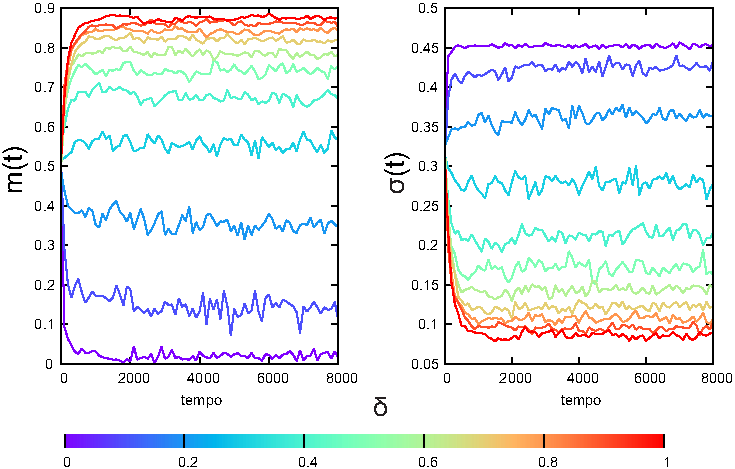
\includegraphics[scale=]{Figures/evolveTermo}
\end{center}
\caption{Figura com a evolução temporal da média e variância entre o alinhamento do agentes e \textit{zeitgeist} para vários valores de $delta$ e com a pressão social $\alpha = 8$, numa rede quadrada com 400 agentes. Até o tempo = 1000, a evolução temporal é feita com o \textit{zeitgeist} fixo, a partir desso ponto a evolução temporal é feita com o \textit{zeitgeist} calculado a partir das médias das opiniões. Percebemos que a evolução dessas grandezas permanece praticamente inalterada com a nova dinâmica.}
\label{fig:evolveTermo}
\end{figure}

Podemos acompanhar o movimento de deriva do \textit{zeitgeist} a partir da figura \ref{fig:evolveAngulosSemFixos} onde mostramos a média do alinhamento entre os agentes e o \textit{zeitgeist} inicial, e o alinhamento entre esse e o \textit{zeitgeist} instantâneo. Observamos nessa figura, que quanto menor o valor do parâmetro $\delta$ mais facilmente os agentes perdem a memória do \textit{zeitgeist} inicial.
\begin{figure}
\begin{center}
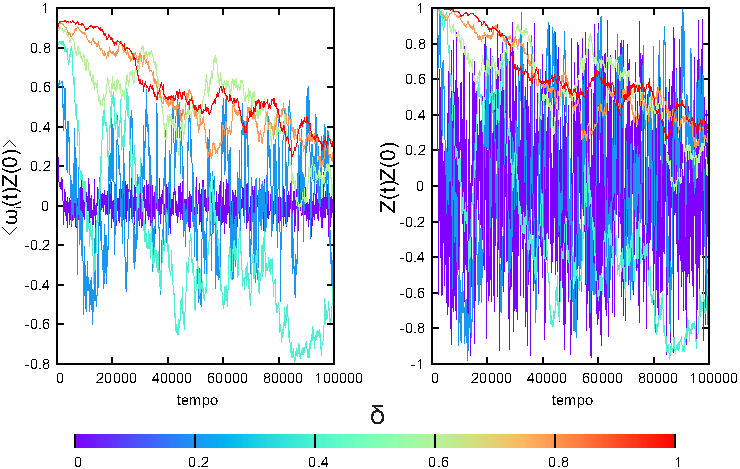
\includegraphics[scale=]{Figures/evolveAngulosSemFixos}
\end{center}
\caption{Figura com movimento de deriva do \textit{zeitgeist}. É mostrado a média do alinhamento dos agentes com o \textit{zeitgeist} inicial, e o produto escalar entre o \textit{zeitgeist} inicial e o instantâneo. Observamos nessa figura, que quanto menor o valor do parâmetro $\delta$ mais facilmente os agentes perdem a memória do \textit{zeitgeist} inicial. Figura simulação feita com 400 agentes dispostos sobre uma rede quadrada.}
\label{fig:evolveAngulosSemFixos}
\end{figure}


O primeiro passo que demos para estudar técnicas de convencimento de população foi supor que na população existia um agente com vetor de opinião fixo $\mathbf{J}_-$ e que não interagia com nenhum outro agente diretamente. A sua ação na sociedade seria dado somente pois a opinião desse agente será contabilizada no calculo do \textit{zeitgeist}, ou seja, 
\begin{equation}
    \mathbf{Z}^t \propto  \sum_{i=1}^k \mathbf{J}_i^t +  \mathbf{J}_-
\end{equation}
Apesar de muito pequena a influência desse agente sobre a sociedade, ele age como um pequeno campo externo que faz com que a sociedade convirja em sua direção para tempos grandes. podemos observar esse efeito na figura \ref{fig:evolveAngulosInit} que mostra a média dos alinhamentos entre as opiniões dos agentes e o \textit{zeitgeist} inicial, e o alinhamento entre o \textit{zeitgeist} instantâneo e a direção do agente fixo, que foi definida na direção oposta ao zeitgeist inicial, $\mathbf{J}_- = - \mathbf{Z}$.
Essa simulação foi feita sobre uma rede quadrada com $400$ agentes interagentes e $1$ agente fixo para vários valores do parâmetro $\delta$.

Portanto, essa simples modificação no modelo nos permitirá estudar uma outra gama de comportamentos sociais, como métodos de convencimento de populações, e talvez nos permita estudar o modelo em outros contextos experimentais, como por exemplo, a disseminação de mensagens em redes sociais como "Facebook","Google+", "Twitter", etc.

\begin{figure}
\begin{center}
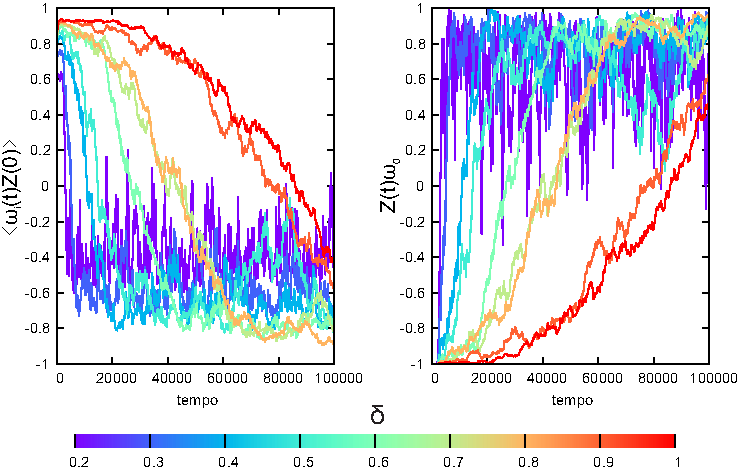
\includegraphics[scale=]{Figures/evolveAngulosInit}
\end{center}
\caption{Figura com a média dos alinhamentos entre as opiniões dos agentes e o \textit{zeitgeist} inicial, e o alinhamento entre o \textit{zeitgeist} instantâneo e a direção do agente fixo, que foi definida na direção oposta ao zeitgeist inicial, $\mathbf{J}_- = - \mathbf{Z}$. Essa simulação foi feita sobre uma rede quadrada com $400$ agentes interagentes e $1$ agente fixo para vários valores do parâmetro $\delta$}
\label{fig:evolveAngulosInit}
\end{figure}

